\documentclass{article}
\usepackage{qilin}
\title{MSE160 Notes}
\author{QiLin Xue}
\lhead{MSE160}
\rhead{QiLin Xue}
\hfuzz=100pt 

\begin{document}
    \maketitle
    \tableofcontents
    \section{Positionality}
\begin{itemize}
    \item A \textbf{position} defines your orientation with respect to an \textbf{entity}.
    \begin{idea}
        How does PIAA affect positionality?
    \end{idea}
    Some ideas from classmates:
    \begin{itemize}
        \item Perception sets initial opinion
        \item You interpret things based on your positionWhat or what you don't perceive affects your positionality.
        \item In breaking the action of perceive-act, you include steps that allow the time to assess your position.
        \item Filters (in perception) depend on position
        \item Understanding your position allows you to assess your interpretations
    \end{itemize}
    \item Subconcious \textbf{bias} will be brought to the table depending on your position, so others can explicityl see how \textit{you} are looking at a situation. 
\end{itemize}
    \section{Lecture 2}
\begin{itemize}
    \item Numbers are \textit{bases} elements of mathematics, so they cannot be defined explicitly in terms of anything more basic. \item Instead they are defined \textit{implicitly}, by imposing the rules, or \textbf{axioms}, that we require they satisfy.
    \begin{idea}
        The axioms are \textit{inspired} by physical reality, but are not \textit{dictated by it}. They do not exist
    \end{idea}
    \item It is important to have as few axioms as possible (to make it philosophically more ``pure'', and to reduce the risk of contradictions:
    \begin{enumerate}
        \item \textbf{Commutative Law}: For each pair $x,y\in \Re$,
        \begin{equation}
            x+y=y+x
            \label{eq:}
        \end{equation}
        and
        \begin{equation}
            xy=yx
            \label{eq:}
        \end{equation}
        \item \textbf{Associative Law}: For each triple $x,y,z \in\Re$,
        \begin{equation}
            x+(y+z)=(x+y)+z
            \label{eq:}
        \end{equation}
        and
        \begin{equation}
            (xy)z=z(yz)
            \label{eq:}
        \end{equation}
        \item \textbf{Distributive Law} For each triple $x,y,z \in \Re$,
        \begin{equation}
            x(y+z)=zy+yz
            \label{eq:}
        \end{equation}
        and
        \begin{equation}
            (x+y)z=xz+yz
            \label{eq:}
        \end{equation}
        \item \textbf{Existence of Identities}: There exists two distinct real numbers, denoted by $0$ and $1$ for which:
        \begin{equation}
            x+0=0+x=x
        \end{equation}
        and
        \begin{equation}
            x\cdot 1 = 1\cdot x=x
            \label{eq:}
        \end{equation}
        for each $x\in \Re$.
        \item \textbf{Existence of inverses} For each $x \in \Re$, there exists a unique additive inverse which we denote by $-x$ for which
        \begin{equation}
            x+(-x)=(-x)+x=0
            \label{eq:}
        \end{equation}
        For each $x\neq 0$ in $\Re$, there exists a unique multiplactive inverse, which we denote by $x^{-1}$ or $1/x$ for which:
        \begin{equation}
            x\cdot \left(x^{-1}\right) = \left(x^{-1}\right)\cdot x=1.
            \label{eq:}
        \end{equation}
        
        
    \end{enumerate}
    \item It's not important to restrict the number of \textbf{definitions}, which are built from axioms, but it gets messy if we make more definitions that are really needed. (e.g. $4 \equiv 3+1$)
    \begin{definition}
        \textbf{Positive integers} are the ``natural numbers'': $1,2,3,\dots$ Note that:
        $$2 \equiv 1+1$$
        and so forth.
    \end{definition}
    \begin{definition}
        \textbf{Rational numbers} are in the form of:
        $$\frac{a}{b} \equiv a \cdot \frac{1}{b}$$
        where $a$, $b$, are integers are $b \neq 0$. Note that this uses axiom 5 with the definition of fractions to create rational numbers.
    \end{definition}
    \item There is no limit to the number of theorems. We can and should prove all \textit{arithmetic} and \textit{algebraic} theorems rigorously logically, starting from the Axioms (e.g. $4=2+2$).
    \begin{example}
        Let us prove $\sqrt{2}$ is irrational by contradiction. Suppose there is a pair of integers: $a$, $b$, such that:
        $$\left(\frac{a}{b}\right)^2=2$$
        where all common factors have been removed.Therefore:
        \begin{align}
            \therefore\,& a^2=2b^2 \\ 
            \therefore\,&a^2 \equiv 0 \pmod{2} \\ 
            \therefore\,&a \equiv 0 \pmod{2} \\ 
        \end{align}
        We can write $a=2q$ where $q$ is some integer such that:
        \begin{align}
            \therefore\,& a^2=4q^2 \\ 
            \therefore\,& 4q^2 = 2b^2 \\ 
            \therefore\,& b^2 = 2q^2 \\ 
            \therefore\,& b^2 \equiv 0 \pmod{2} \\ 
            \therefore\,& b \equiv 0 \pmod{2}
        \end{align}
        However, since $a$ and $b$ are both even, we have contradicted our statement that all common factors have been removed. Thus $\sqrt{2}$ cannot be rational and can only be irrational.
    \end{example}
    \item However, the 5th field axiom only discusses the creation of rational numbers. We could simply add a ``root 2 axiom'' to create $\sqrt{2}$, just like we did for $0$ and $1$.
    \vspace{2mm}

    \item This is super messy because it would imply we'd need another axiom for every irrational, including every root of every \textbf{polynomial function}:
        \begin{equation}
            P_n(x)=a_nx^n+a_{n-1}x^{n-1}+\cdots+a_1x+a_0
            \label{eq:}
        \end{equation}
    where $a$ can be any specified number and $n$ is a positive integer. If we set $P_n(x)=0$, we get a polynomial equation where we can find the roots.
    \begin{definition}
        If $z$ is a root of $p_n(x)$ then $p_n(z)=0$.
    \end{definition}
    There are $n$ roots\footnote{Per the fundamental theorem of algebra, which is beyond the scope of this course}, most are irrational and are called \textbf{algebraic numbers}.
    \item To prevent creating numerous new axioms, we create a new axiom called \textbf{CORA}: Completeness of the Reals Axiom, which tells us that every non-empty set of real numbers that is bounded above has a least upper bound among the real numbers.
    \begin{definition}
        A set of real numbers, $\mathbb{S}$ is bounded above if and only if there exists some number $M$ such that $x \le M$ for all $x \in \mathbb{S}$. For example:
        \begin{equation}
            \mathbb{S}_1=\{1,3,\frac{17}{5},211\}
            \label{eq:}
        \end{equation}
        Here, $M=211$ or $250$, etc. We can write the first upper bound as:
        \begin{equation}
            \mathrm{ub}\mathbb{S}_1=211
            \label{eq:}
        \end{equation}
    \end{definition}
    \begin{definition}
        The least upper bound is the smallest of all the upper bounds. Here:
        \begin{equation}
            \mathrm{lub}\mathbb{S}_1=211
            \label{eq:}
        \end{equation}
    \end{definition}
    \item Note that we \textbf{do not} require that $\mathrm{lub}\mathbb{S} \in \mathbb{S}$ necessarily. For example, if:
    \begin{equation}
        \mathbb{S}_2 = \{x:x^2<2\}
        \label{eq:}
    \end{equation}
    There are several upper bounds in this set, but is there a least upper bound? We may think intuitively it is $\sqrt{2}$, but we have to be careful! We haven't proved it exists yet. \textbf{However,} CORA has \textit{creates} this new number, $\sqrt{2}$, by demanding that it exists.\footnote{However, proving that the lower upper bound is $\sqrt{2}$ is rather tricky and was removed from the supplement.}
    \item Additionally, CORA does the same for all \textbf{algebraic irrationals} and \textbf{transcendental irrationals}. Without CORA, there would be no irrational numbers!
\end{itemize}
    \section{Integration}
\subsection{Recap of Integration}
\begin{itemize}
    \item The definite integral has the geometric interpretation as the area under the curve $f(x)$ between $x=a$ and $x=b$ and the $x$ axis:
    \begin{equation}
        \int_a^b f(x) \dd{x}
    \end{equation}
    but can be rigorously defined using a Riemann sum:
    \begin{equation}
        \int_a^b f(x) \dd{x} \equiv \lim_{\Vert P \rVert} \sum_{i=1}^n f(x_i^*)\Delta x_i
        \label{eq:}
    \end{equation}
    Often, we have a uniform partition, such that $\Delta x_i = \frac{b-a}{n}$ where $n$ is the number of partitions. And if we choose to use the right hand endpoint, then:
    \begin{equation}
        f(x_i^*) = f(x_i) = f(x_i) = f\left(a+\frac{b-a}{n}i\right)
    \end{equation}
    \begin{example}
        To solve $\int_0^5 x^2 \dd{x}$, we can choose a uniform partition with:
        \begin{equation}
            \Delta x = \frac{5-0}{n} = \frac{5}{n}
        \end{equation}
        and:
        \begin{equation}
            x_i^* = x_i = i\Delta x \implies f(x_i^*)=(i\Delta x)^2 = \left(i\frac{5}{n}\right)^2
        \end{equation}
        The area approximation is:
        \begin{align}
            A \simeq \sum_{i=1}^n \Delta x_i f(x_i^*) &= \sum_{i=1}^n \left(\frac{5}{n}\right)\left(i\frac{5}{n}\right)^2 \\ 
            &= \frac{125}{n^2} \sum_{i=1}^n i^2 = \frac{125}{n^3} \frac{n(n+1)(2n+1)}{6}
        \end{align}
        Taking the limit as $n\to \infty$, we get:
        \begin{equation}
            \int_0^5 x^2 \dd{x} =  \lim_{n\to\infty} \frac{125}{6}\left(2+\frac{2}{n}+\frac{1}{n^2}\right) = \frac{5^3}{3}.
        \end{equation}
    \end{example}
    \begin{example}
        To evaluate $\int_1^2 x^{-2} \dd{x}$, we can choose
        \begin{equation}
            x_i^* = \sqrt{x_{i-1}x_i}
        \end{equation}
        and a uniform partition of:
        \begin{equation}
            \Delta x = \frac{2-1}{n} = \frac{1}{n}
        \end{equation}
        such that:
        \begin{equation}
            x_i = 1+i\Delta x = 1 + \frac{i}{n} = \frac{n+i}{n}
        \end{equation}
        and
        \begin{equation}
            x_{i-1} = \frac{n+i-1}{n}
        \end{equation}
        such that the area is:
        \begin{align*}
            A &\simeq \sum_{i=1}^n \Delta xf(x_i^*) \\ 
            &= \sum_{i=1}^n \frac{1}{n} \left(\frac{1}{x_i^*}\right)^2 \\ 
            &= \sum_{i=1}^n \frac{1}{n} \frac{1}{x_{i-1}x_i} \\ 
            &= \sum_{i=1}^n \frac{1}{n} \frac{n}{n+i-1}\cdot \frac{n}{n+i} \\
            &= \sum_{i=1}^n n \frac{1}{n+i-1} \cdot \frac{1}{n+i} \\ 
            &= \sum_{i=1}^n \left(\frac{1}{n+i-1}-\frac{1}{n+i}\right) \\ 
            &= n\left[\sum_{i=1}^n \frac{1}{n+i-1} - \sum_{i=1}^n \frac{1}{n+i}\right] \\ 
            &= n\left[\sum_{i=0}^n \frac{1}{n+i} - \sum_{i=1}^n \frac{1}{n+i}\right] \\ 
            &= n\left[\frac{1}{n}+\frac{1}{n+1}+\frac{1}{n+2}+\cdots+\frac{1}{2n-1}-\frac{1}{n+1}-\frac{1}{n+2}-\cdots-\frac{1}{2n}\right] \\ 
            &=n\left(\frac{1}{n}-\frac{1}{2n}\right) \\ 
            &= 1 - \frac{1}{2} = \frac{1}{2}
        \end{align*}
        The part where we cancel out everything is called a \textbf{telescoping series}. Notice how the area doesn't depend on $n$ so we get the exact area, even if we let $n=1$!.
    \end{example}
    \item We need a better way to do integration, so we can define:
    \begin{equation}
        F(x) \equiv \int_a^x f(t) \dd{t}
    \end{equation}
    such that $F'(x) = f(x)$. This is the definition of the antiderivative. This leads to the fundamental theorem of calculus:
    \begin{equation}
        \int_a^b f(t) \dd{t} = F(h) - F(a)
    \end{equation}
    and the indefinite integral can be written as:
    \begin{equation}
        \int f(x) \dd{x} = G(x) + C
    \end{equation}
    The main problem now becomes trying to \textit{find antiderivatives}, which is much easier than Riemann sums, though still more difficult than calculating derivatives.
\end{itemize}
\subsection{Techniques of Integration}
\begin{itemize}
    \item \textbf{Integration by Parts} attempts to reverse the product rule:
    \begin{equation}
        (fg)' = fg' + f'g
    \end{equation}
    Taking the integral of both sides gives:
    \begin{align}
        f(x)g(x) &= \int f(x)g'(x) \dd{x} + \int f'(x) g(x) \dd{x} \\ 
        \int f(x)g'(x) \dd{x} &= \int f(x) g'(x) \dd{x} = f(x)g(x) - \int f'(x)g(x) \dd{x}
    \end{align}
    If the second integral is easier than the first, then we have made substaintial progress.
    \begin{idea}
        Integration of parts tells us that:
        \begin{equation}
            \int u \dd{v} = uv - \int v \dd{u}
        \end{equation}
    \end{idea}
    \begin{example}
        To solve $\int xe^{2x}$, we can let:
        \begin{align}
            &u=x            &\dd{v} = e^{2x} \dd{x} \\ 
            &\dd{u}=\dd{x} &v=\frac{1}{2}e^{2x} 
        \end{align}
        which gives:
        \begin{align}
            & \frac{1}{2}xe^{2x} - \int \frac{1}{2}e^{2x} \dd{x} \\ 
            &= \frac{1}{2}xe^{2x} - \frac{1}{4}e^{2x} + C
        \end{align}
        We can check:
        \begin{align}
            \frac{d}{dx}\left(\frac{1}{2}xe^{2x}-\frac{1}{4}e^{2x}+C\right) \\ 
            &= xe^{2x} + \frac{1}{2}e^{2x}-\frac{2}{4}e^{2x} \\ 
            &= xe^{2x}
        \end{align}
    \end{example}
    \begin{example}
        To solve $\int x^2\sin(2x) \dd{x}$, we let:
        \begin{align}
            &u=x^2            &\dd{v} = \sin 2x\dd{x} \\ 
            &\dd{u}=2x\dd{x} &v=-\frac{1}{2}\cos(2x) 
        \end{align}
        which gives:
        \begin{equation}
            =-\frac{1}{2}x^2\cos 2x + \int x\cos(2x) \dd{x}
        \end{equation}
        and we can apply integration by parts a second time, if we let:
        \begin{align}
            &u=x            &\dd{v} = \cos 2x\dd{x} \\ 
            &\dd{u}=\dd{x} &v=\frac{1}{2}\sin(2x) 
        \end{align}
        which gives us:
        \begin{align}
            &=-\frac{1}{2}x^2\cos(2x) + \frac{1}{2}x\sin(2x) - \int \frac{1}{2}\sin(2x) \dd{x} \\ 
            &=-\frac{1}{2}x^2\cos(2x)+\frac{1}{2}x\sin(2x) +\frac{1}{4}\cos(2X)+C
        \end{align}
    \end{example}
    \begin{example}
        To solve $I=\int e^{x}\sin x\dd{x}$, we can let:
        \begin{align}
            &u=\sin x            &\dd{v} =e^x\dd{x} \\ 
            &\dd{u}=\cos x\dd{x} &v=e^x
        \end{align}
        to give us:
        \begin{equation}
            = e^x\sin x - \int e^{x}\cos x \dd{x}
        \end{equation}
        We apply integration by parts a second time:
        \begin{align}
            &u=\cos x            &\dd{v} =e^x\dd{x} \\ 
            &\dd{u}=-\sin x\dd{x} &v=e^x
        \end{align}
        to get:
        \begin{align}
            I&=e^x\sin x - e^x\cos x - \underbrace{\int e^x\sin x \dd{x}}_{I} \\ 
            2I &= e^x\left(\sin x - \cos x\right) + C' \\ 
            I &= \frac{1}{2}e^x\left(\sin x - \cos x\right) + C
        \end{align}
        and we are done.
    \end{example}
    \begin{example}
        We can also solve integrals that do not appear to have parts, such as $\int \ln x \dd{x}$. We choose:
        \begin{align}
            &u=\ln x            &\dd{v} =\dd{x} \\ 
            &\dd{u}=\frac{1}{x}\dd{x} &v=x
        \end{align}
        to give us:
        \begin{equation}
            \ln x - \int \dd{x} = x\ln x - x + C
        \end{equation}
    \end{example}
    \item For a definite integral, we can write IBP as:
    \begin{equation}
        f(x)g(x)\Big|^b_a-\int_a^b f'(x)g(x) \dd{x}
    \end{equation}
    \begin{example}
        It is \textit{possible} to apply integration of parts to find the integral of $\int \tan x \dd{x} = \int \frac{\sin x}{\cos x} \dd{x}$. We can let:
        \begin{align}
            &u=\frac{1}{\cos x}=\sec x            &\dd{v} =\sin x\dd{x} \\ 
            &\dd{u}=\sec x\tan x &v=-\cos x
        \end{align}
        this gives us:
        \begin{align}
            \int \tan x \dd{x} &= -\frac{\cos x}{\cos x}+ \int \tan x \dd{x}
        \end{align}
        Notice that we could try to subtract the original integral from both sides and get:
        \begin{equation}
            0 = -1
        \end{equation}
        which is clearly wrong! However, we forgot the constant of integration, so the correct statement would be:
        \begin{equation}
            0 + C' = -1 + C
        \end{equation}
        which does not tell us anything interesting.
    \end{example}
\end{itemize}

    \section{Lecture 4: Projections}
\begin{itemize}
    \item For two nonzero vectors $\vec{v}$ and $\vec{w}$ such that:
    \begin{equation}
        \vec{v}\cdot\vec{w}=0\implies \cos\theta=0\implies \theta=\frac{\pi}{2}
        \label{eq:}
    \end{equation}
    If $\vec{v}$ and/or $\vec{w}$ is the zero vector,
    \begin{equation}
        \vec{v}\cdot\vec{w}=0
        \label{eq:}
    \end{equation}
    is also true.
    \begin{definition}
        $\vec{v}$ and $\vec{w}$ are orthogonal if and only if $\vec{v}\cdot\vec{w}=0$.
    \end{definition}
    \item Projections are what we use to define points in 2-d and 3-d. For example:
    \begin{center}
        \begin{tikzpicture}
            \draw[->] (0,0) -- (5,0) node[right] {$x$};
            \draw[->] (0,0) -- (0,5) node[right] {$y$};

            \draw[thick,->] (0,0) -- (3,4) node[right] {$(v_1,v_2)$};
            \draw[dotted] (0,4) node[left] {$(0,v_2)$} -- (3,4);
            \draw[dotted] (3,0) node[below] {$(v_1,0)$} -- (3,4);

            \draw[very thick,->] (0,0) -- (1,0) node[midway,below] {$\vec{i}=\begin{bmatrix}
                1\\0
            \end{bmatrix}$};
            \draw[very thick,->] (0,0) -- (0,1) node[midway,left] {$\vec{j}=\begin{bmatrix}
                1\\0
            \end{bmatrix}$};

            \draw[thick,->] (0,0) -- (0,3);
            \draw[thick,->] (0,0) -- (4,0);
        \end{tikzpicture}
    \end{center}
    We can write $\vec{v}=\begin{bmatrix}
        v_1\\v_2
    \end{bmatrix}$ as:
    \begin{align}
        \vec{v} &= v_1\vec{i}+v_2\vec{j} \\ 
        &= v_1\begin{bmatrix}
            1\\0
        \end{bmatrix} + v_2\begin{bmatrix}
            0\\ 1
        \end{bmatrix}
        \\ 
        &= \begin{bmatrix}
            v_1\\v_2
        \end{bmatrix}
    \end{align}
    \item Let's generalize this concept to project one vector $\vec{w}$ on another vector $\vec{v}$
    \begin{center}
        \begin{tikzpicture}
            \draw[thick,->] (0,0) -- (8,2) node[right] {$\vec{v}$};
            \draw[thick,->] (0,0) -- (3,3) node[right] {$\vec{w}$};
            \draw[very thick,->] (0,0) -- (3.53,0.88) node[midway,below] {$\vec{u}$};
            \draw[dotted] (3,3) -- (3.53,0.88);
        \end{tikzpicture}
    \end{center}
    We can say that: $\vec{u}$ is the projection of $\vec{w}$ on $\vec{v}$. Based on the way we have constructed $\vec{u}$ we know it has certain properties:
    \begin{itemize}
        \item $\vec{u}$ is parallel to $\vec{v}$, so it can be expressed as a multiple of $\vec{v}$ such that:
        \begin{equation}
            \vec{u}=c\vec{v}
            \label{eq:}
        \end{equation}
        where $c$ is a scalar.
        \item We can say that $\vec{w}-\vec{u}$ (and by extension $\vec{u}-\vec{w}$) is orthogonal to $\vec{v}$:
        \begin{equation}
            (\vec{w}-\vec{u})\cdot \vec{v}=0
            \label{eq:}
        \end{equation}
    \end{itemize}
    Using these two properties, we can solve for the unknown $c$:
    \begin{align}
        (\vec{w}-\vec{u})\cdot \vec{v} &= 0 \\
        \vec{w}\cdot\vec{v}-\vec{u}\cdot\vec{v} &= 0 \\
        \vec{w}\cdot\vec{v}-(c\vec{v})\cdot\vec{v} &= 0 \\ 
        \vec{w}\cdot\vec{v}-c\left(\vec{v}\cdot\vec{v}\right) = 0 
    \end{align}
    Solving for $c$ gives:
    \begin{equation}
        c=\frac{\vec{w}\cdot\vec{v}}{\vec{v}\cdot\vec{v}}
        \label{eq:}
    \end{equation}
    so we have:
    \begin{equation}
        \boxed{\vec{u}=\frac{\vec{w}\cdot\vec{v}}{\vec{v}\cdot\vec{v}}\vec{v}}
        \label{eq:}
    \end{equation}
    \begin{definition}
        The projection of $\vec{w}$ on $\vec{v}$ can be written as:
        \begin{equation}
            \vec{u}=\text{proj}_{\vec{v}}\vec{w}
            =
            \frac{\vec{w}\cdot\vec{v}}{\vec{v}\cdot\vec{v}}\vec{v}
            = \frac{\vec{w}\cdot\vec{v}}{\lVert \vec{v} \rVert^2} \vec{v}
            = \frac{\vec{w}\cdot\vec{v}}{\lVert \vec{v} \rVert} \frac{1}{\lVert\vec{v}\rVert}\vec{v}
            \label{eq:}
        \end{equation}
        where the last part $\frac{1}{\lVert\vec{v}\rVert}\vec{v}$ is a unit vector pointing in the direction of $\vec{v}$.
    \end{definition}
    \item Suppose we wish to project a vector $\vec{v}$ onto another vector (e.g. z-axis) in three dimensions. \textit{The same formula applies.}
    \item Suppose instead we wish to project $\vec{v}$ on a plane, such as the xy plane? If $\vec{v}=\begin{bmatrix}
        v_1\\v_2\\v_3
    \end{bmatrix}$. Then the projection would be $\begin{bmatrix}
        v_1\\v_2\\0
    \end{bmatrix}$.
\end{itemize}
    \section{Lecture 5}
\begin{itemize}
    \item There is a linear relationship between the force of a wire and the deformation. The slope was called the stiffness:
    \begin{equation}
        k = \frac{F}{\Delta L}
        \label{eq:}
    \end{equation}
    The problem with this is that the slope would be different for different sizes of the same object, so it didn't reflect a particular object's characteristics.
    \item Young modified this relationship to instead measure the tensile strength $\sigma=F/A$ in terms of the strain $\epsilon=\frac{\Delta L}{L}$, such that:
    \begin{equation}
        E = \frac{\sigma}{\epsilon}
        \label{eq:}
    \end{equation}
    This provides a method to experimentally determine the value of $E$, by loading different weights and measuring the strain for each.
    \item A \textbf{Coupon Test} is the testing of a small representative piece of a material to determine the properties. We do this via the setup below, where we place two indicators a length $L_0$ apart. As we load weight onto the rectangle, the distance between the indicators will change to $L_0+\Delta L$.
    \begin{center}
        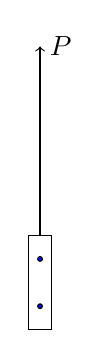
\begin{tikzpicture}[scale=0.3]
            \draw[] (-0.5,2) rectangle (0.5,-2);
            \draw[fill=blue] (0,1) circle (0.1);
            \draw[fill=blue] (0,-1) circle (0.1);
            \draw[->] (0,2) -- (0,10) node[right] {$P$};
        \end{tikzpicture}
    \end{center}
    \item We can increase the strain by adding weights below and measuring the force $P$. Dividing it through by the area gives the tensile strength.
    \begin{center}
        \begin{tikzpicture}
            \coordinate (O) at (0,0);
            \draw[->] (O) -- (12,0) node[above] {$\epsilon$};
            \draw[->] (O) -- (0,6);
            
            \draw[<->,dotted] (0,2.5) -- (3,2.5) node[midway,above] {$\text{linear elastic}$};
            \draw[] (O) -- (3,2);

            \draw[<->, dotted] (3,2.5) -- (6,2.5) node[midway,above] {$\text{yield plateau}$};
            \draw[] (3,2) -- (6,2);
            \draw[dotted] (3,2) -- (0,2) node[left] {$\sigma_{yield}$};
            \draw (0,4) node[left] {$\sigma_{ultimate}$};

            \draw[] (9,4) parabola (6,2);
            \draw[<->, dotted] (6,2.5) -- (9,2.5) node[midway,above] {$\text{strain hardening}$};
            \draw[] (9,4) parabola (11,3);
            \draw[<->, dotted] (9,2.5) -- (11,2.5) node[midway,above] {$\text{necking}$};

        \end{tikzpicture}
    \end{center}
    \item The \textbf{yield plateau} occurs when the atoms in the metal are no longer vibrating back and forth between one another, but sliding across one another. As a result, we experience \textbf{permanent plastic deformations} during this period.
    \item At a certain point, the imperfections build up such that yielding becomes more difficult, so in order to overcome them, the stress increases. This process is known as \textbf{strain hardening}.
    \item \textbf{Necking} occurs after the ultimate stress point where the cable will form a neck shape, reducing the tensile strength.
    \item \textbf{Rupture} occurs after the cable cannot support the strain at all and then break.
    \item If the applied load is taken off, the cable will contract back to $\sigma=0$ following the same slope. After the initial yield plateau, the cable will not be able to naturally go back to its original rest length.
\end{itemize}
    \newpage
    \section{Lecture Six: Stress-Strain Response}
\begin{itemize}
    \item For a \textbf{brittle} material, the slope of the stress-strain graph will be very high and it will have almost no warning before breaking.
    \begin{itemize}
        \item Applications: Piano wires
    \end{itemize}
    \item Other wires, such as \textbf{flossing wires}, which are used to reinforce concrete, there is a different behaviour, where yielding occurs very early.
    \begin{center}
        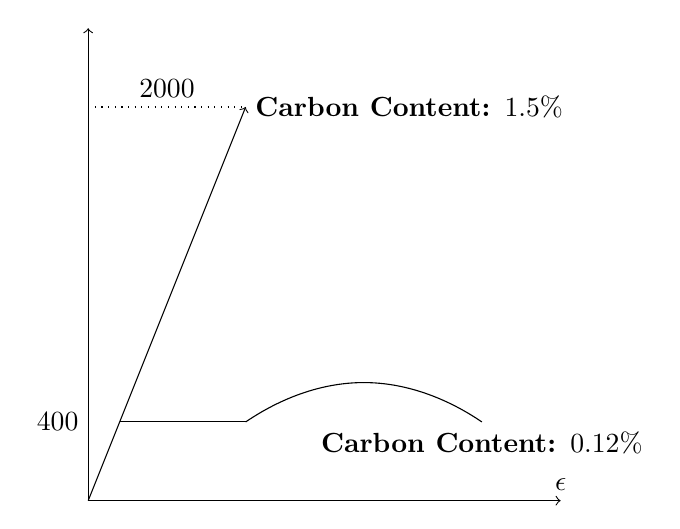
\begin{tikzpicture}
            \coordinate (O) at (0,0);
            \draw[->] (O) -- (6,0) node[above] {$\epsilon$};
            \draw[->] (O) -- (0,6);
            \draw[] (0,1) node[left] {$400\si{\mega\pascal}$};
            \draw[dotted] (0,5) -- (2,5) node[midway,above] {$2000\si{\mega\pascal}$};
            \draw[->] (O) -- (2,5) node[right] {$\textbf{Carbon Content: }1.5\%$};

            \draw[] (0.4,1) -- (2,1);
            \draw[] (3.5,1.5) parabola (2,1);
            \draw[] (3.5,1.5) parabola (5,1) node[below] {$\textbf{Carbon Content: }0.12\%$};
        \end{tikzpicture}
    \end{center}
    \item \textbf{Work} is defined as:
    \begin{equation}
        \text{Work} = \text{Force} \cdot \text{Distance}
        \label{eq:}
    \end{equation}
    and is measured in Joules ($[\si{\joule}]=[\si{\newton\meter}]$) and \textbf{energy} is defined as the capacity to do work
    \item Body fat can store around $40\si{\mega\joule\per\kilogram}$ in body fat, where $7.5\%$ of it can be transferred. One rule of thumb is that one pound of body fat carries you $35$ miles.
    \item Power is the rate at which work is being done. Originally defined as:
    \begin{equation}
        1\text{ HP} = 746\si{\watt}
        \label{eq:}
    \end{equation}
    \item The work, or energy stored in deforming a wire is the area under the curve of the force vs displacement curve. The \textbf{elastic strain energy} gives the maximum recoverable energy, or:
    \begin{equation}
        E=\frac{1}{2}F_\text{max}\Delta_\text{max} = \frac{1}{2}\sigma A \times \epsilon L
        \label{eq:}
    \end{equation}
    The energy density is:
    \begin{equation}
        E/V = \frac{1}{2}\sigma\epsilon
        \label{eq:}
    \end{equation}
    \item The resilience of a material is directly related to its ability to store elastic strain energy.
    \item Some vocabulary terms:
    \begin{itemize}
        \item Weight $[\si{\kilo\newton\per\meter\cubed}]$ - weight density of the material
        \item Stiffness $E[\si{\mega\pascal}]$ - The Young's Modulus: How difficult it is to stretch
        \item Tensile strength $[\si{\mega\pascal}]$- Critical points at which the material starts to yield, or break (ultimate).
        \item Compressive strength  $[\si{\mega\pascal}]$ - yield strength equivalent of tensile strength, except for compressions.
        \item Resilience $[\si{\mega\joule\per\meter\cubed}]$ - maximum energy which a material can absorb per unit volume before experiencing permanent deformations.
        \item Toughness $[\si{\mega\joule\per\meter\cubed}]$ - maximum energy which a material can absorb per unit volume before experiencing permanent deformations.
        \item Ductility is the maximum elongation before it experiences failure.
        \item $\alpha[10^{-6} \si{\per\celsius}]$ - thermal expansion coefficient
    \end{itemize}
\end{itemize}
    \section{Technical Mechanical Behaviour}
\begin{itemize}
    \item The ultimate tensile strength, denoted as $UTS$ or $\sigma_\text{UTS}$ is the highest stress that a material can occur in a material.
    \item The \textit{proportional limit} describes the point on the tensile stress-strain curve where elastic deformations no longer occur.
    \item Along with the yield strength, it is difficult to define this objectively. Instead, we use the following convention:
    \begin{definition}
        The yield strength is the stress value at which if the material is unloaded at that point, the strain will be $\epsilon = 0.002 = 0.2\%$.
    \end{definition}
    \item Uniform deformation occurs when the thickness of the material is uniform. Non-uniform deformation occurs when an increase in strain results in a decrease in stress. This is known as \textbf{necking}.
\end{itemize}
    \section{Polymers}
\begin{itemize}
    \item A useful analogy for polymers is to imagine a \textit{molecular hand}. A polymer is consisted of several twisted and tangled chains of molecules. This is known as \textit{entanglement}. This is due to the non-linear nature of the polymers and the fact that bonds can rotate.
    \item To plastically deform a polymer, we can imagine a microscopic hand pulling a polymer. If you are able to do so, then it is seen as plastic deformation
    \item The molecular chains are connected via weak intermolecular forces. Increasing the temperature increases the vibration, allowing the molecular hand to more easily separate them.
    \begin{idea}
        When a polymer undergoes a physical transformation (i.e. melting, dissolving, deforming), it is due to the intermolecular interactions, not the intramolecular interactions. 
    \end{idea}
    \begin{case}
        Plastic exhibits very interesting behaviour when it is stretched. During plastic deformation, the molecules can line up, which can cause the following physical changes:
        \begin{itemize}
            \item Color change (lighter)
            \item Strong in the direction of stretching
            \item Weaker in the direction perpendicular to stretching
        \end{itemize}
        The polymers become \textit{oriented} (also known as \textit{conditioned}) with the loading axis. This is a great demonstration that shows how polymers can be thought of as an interconnected mix of long polymer chains.
    \end{case}
    \item We define the yield strength as the point in which necking occurs (first local maximum in the stress-strain curve)
    \subsection{Chemical Basics}
    \item To describe the polymers on a molecular level, we look at it from an organic chemistry perspective. Instead of unit cells, we look at \textit{mer} units (the suffix of \textit{polymer}), which is the starting molecule when building the polymer.
    \begin{case}
        Polyethylene (PE) is a polymer that is consisted of ethene (or more commonly known as ethylene), shown below:
        \begin{center}
            \chemfig{C(-[3]H)(-[5]H) =   C(-[1]H)(-[7]H)}
        \end{center}
        and polyethylene looks like:
        \begin{center}
            \chemfig{-C(-[2]H)(-[6]H)-[@{op,.75}]C(-[2]H)(-[6]H)-C(-[2]H)(-[6]H)-[@{cl,0.25}]C(-[2]H)(-[6]H)-}
            \polymerdelim[height = 5pt, indice = \!\!]{op}{cl}
        \end{center}
        \vspace{2mm} % weird space, don't know why this is the case
        Notice the absence of the double bond. This is due to the chemical reaction that is required to take the mer unit and add it to the polymer.
    \end{case}
    \item Here are some other examples:
    \begin{itemize}
        \item  Polypropylene (PP) is a very common polymer used in many areas (e.g. Starbucks reusable cups). It is a material that is generally stronger and has a higher elastic modulus than polyethylene. This is because it has an extra \ch{CH3} methyl group, as shown below:
        \begin{center}
            \chemfig{-[@{op,.75}]C(-[2]H)(-[6]H)-C(-[2]H)(-[6]CH_3)-[@{cl,0.25}]}
            \polymerdelim[height = 5pt, indice = \!\!]{op}{cl}
        \end{center}
        \item Polyvinylchloride (PVC), along with PE and PP are the three most produced polymers in the world. The structure is similar, except with a chloride atom in the monomer unit:
        \begin{center}
            \chemfig{-[@{op,.75}]C(-[2]H)(-[6]H)-C(-[2]H)(-[6]Cl)-[@{cl,0.25}]}
            \polymerdelim[height = 5pt, indice = \!\!]{op}{cl}
        \end{center}
        The term \textit{vinyl} describes two carbon atoms connected via double bond.
    \begin{case}
        PVC is very strong and has a high elastic modulus. We can explain this by looking at the chemical properties of the chloride atom. Chlorine is an extremely electronegative atom, meaning it tends to attract electrons. This allows it to attract electrons from the hydrogen of neighbouring polymers, forming a hydrogen bond\footnote{Hydrogen bonds are actually much more complicated than this, but this isn't a chemistry course.} This forms a dipole moment, which can be illustrated below via the following notation:
        \vspace{4mm}
        \begin{center}
            \chemfig{
                \chemabove[3pt]{H}{\scriptstyle\delta^+}(-[::270,0.5,,,draw=none]@{c})-
                \chemabove[3pt]{Cl}{\scriptstyle\delta^-}(-[::270,0.5,,,draw=none]@{d})
               }
               \chemmove{
                       \draw[|->] (c)--(d);
               }
        \end{center}
        \vspace{2mm}
        The $\delta^+$ and $\delta^-$ signify the \textit{partial charges} and the arrow is the shorthand notation for the direction of the dipole (which will always point in the direction a proton would move in)
        \vspace{2mm}

        Since this bond is so strong, it is harder for nearby polymers to move against each other due to stronger intermolecular forces. Similarly, PP is strong for similar chemical properties. However instead of hydrogen bonds, it is the extra methyl group increasing london dispersion forces between neighbouring gorups.
    \end{case}
    \item Polytetrafluoroethylene (PTFE) is used for non-stick surfaces. As a result, it is very non-reactive, and it is able to do so due to the large fluorine atoms bonded to each carbon:
    \begin{center}
        \chemfig{-[@{op,.75}]C(-[2]F)(-[6]F)-C(-[2]F)(-[6]F)-[@{cl,0.25}]}
        \polymerdelim[height = 5pt, indice = \!\!]{op}{cl}
    \end{center}
    Their large size helps protect intramolecular bonds within PTFE from being broken and although they are highly electronegative, they are actually nonpolar due to its symmetry.
    \item Polymethylmethacrylate (PMMA) are often used for windows because they can be made optically transparent. The reason they are transparent is because of a bulky side group in their monomer unit that prevents close packing of polymer chains, creating an \textit{amorphous} structure.
    \begin{center}
        \chemfig{-[@{op,.75}]C(-[2]F)(-[6]F)-C(-[2]F)(-[6]C(=[0]O)(-[6]O(-[6]CH_3)))-[@{cl,0.25}]}
        \polymerdelim[height = 5pt, indice = \!\!]{op}{cl}
    \end{center}
    \begin{case}
        We investigate what makes a material transparent, translucent, and opaque from a materials science perspective Polymers can easily align with one another and become organized, which is known as crystallization. When it crystallizes, the index of refraction is different from when it is amorphous. Therefore, if it contains parts that are both amorphous and crystalline (known as \textit{semicrystalline}), the light will not follow a direct path and the polymer will become translucent or opaque.
        \vspace{2mm}

        So how do we make a polymer transparent? If it is completely crystalline, then it would be transparent but polymers can never be 100\% crystalline. Instead, we want them to be 100\% amorphous.
        \vspace{2mm}

        Moving away from the domain of polymers, sapphire has a crystalline structure, made of $Al_2O_3$, and is clear and transparent. Window glass made from silica is amorphous and also clear and transparent. While polycrystalline metals are opaque, we can also have glassy metals, but they are also opaque. To get the full picture, we need a better understanding of how light works.
    \end{case}
    \end{itemize}
    \item To draw bonds going out and in of the page, we use a shaded triangle and dashed triangle, respectively. For example, we would draw methane as:
    \begin{center}
        \chemfig{C(<:[-0.3]H)(<[-1.1]H)(-[2]H)(-[5]H)}
    \end{center}
    \item We often use the symbol $R$ to denote an arbitrary functional group.
    \subsection{Length}
    \item We can characterize the length of a polymer with its linear mass density and the total mass.
    \begin{case}
        Ultrahigh Molecular Weight Polyethylene is often used in hip replacements. It often replaces part of the hip to prevent parts of it from wearing it away. It has high strength, high tolerance, and biocompatible.
        \vspace{2mm}

        As we increase molecular weight in a polymer, we increase the strength and typically increase the strain to fracture due to the increased entanglement of the long molecules.
    \end{case}
    \item The \textbf{number average molecular weight} can be defined as:
    \begin{equation}
        \overline{M}_\text{number} = \sum_{n=1}^i M_nx_n
    \end{equation}
    for a polymer containing $i$ groups where $M_n$ is the molecular weight of the $n^\text{th}$ group and $x_n$ is the number fraction of the $n^\text{th}$ group.
    \item Similarly, the \textbf{weight average molecular weight} can be defined as:
    \begin{equation}
        \overline{M}_\text{weight} = \sum_{n=1}^i M_nw_n
    \end{equation}
    where $w_n$ is the weight fraction of the $n^\text{th}$ group. The weight average will always be larger (and maintains equality) than the number average.
    \begin{proof}
        Suppose we have $i$ groups with molecular weights of $\{M_1, M_2, \dots, M_n\}$ and number fractions of $\{x_1, x_2, \dots \}$. We can calculate the weight fraction to be:
        \begin{equation}
            w_n = \frac{M_nx_n}{M_1x_1+M_2x_2 + \cdots +M_ix_i} = \frac{M_nx_n}{\overline{M}_\text{number}}
        \end{equation}
        so we have:
        \begin{equation}
            \overline{M}_\text{weight} = \frac{1}{\overline{M}_\text{number}}\sum_{n=1}^i  M^2_nx_n
        \end{equation}
        We propose that $\overline{M}_\text{number} \le \overline{M}_\text{weight}$ such that:
        \begin{align}
            \overline{M}_\text{number} & \le  \frac{1}{\overline{M}_\text{number}}\sum_{n=1}^i  M^2_nx_n \\ 
            \overline{M}^2_\text{number} &\le \sum_{n=1}^iM^2_nx_n \\ 
            \sum_{n=1}^i M_nx_n &\le \sqrt{\sum_{n=1}^i M^2_nx_n}
        \end{align}
        The right hand side gives the RMS average and the left hand side gives the arithmetic average. According to the \href{https://en.wikipedia.org/wiki/HM-GM-AM-QM\_inequalities}{RMS-AM inequality}, the RMS mean is always greater or equal to the arithmetic mean.
    \end{proof}
    This \textbf{disparity} is actually quite important, and is also known as the \textbf{polydisperity index} and is defined as:
    \begin{equation}
        \text{\DJ} = \frac{\overline{M}_\text{weight}}{\overline{M}_\text{number}}
    \end{equation}
    \subsection{Close Packing and Crystallization}
    \item As polymer chains line up, the density can increase. Since the chains get closer together, the strength of the intermolecular interactions may also increase, increasing the elastic modulus.
    \item When polymers line up, they form a crystalline structure (i.e. zigzag pattern). However, there will always still be some amorphous sections. As a result, there is an incentive to increase crystallinity and this can be accomplished by having simple mer units and regular repeating structures.
    \item When functional groups are on the same side, such as shown below, it is easier for the polymer to have a close packing behaviour:
    \begin{center}
        \chemfig{[-0.3]-C(<[-1.6]R)(<:[5.6]H)-[0.3]C(<[-1.6]R)(<:[5.6]H)-[-0.3]C(<[-1.6]R)(<:[5.6]H)-[0.3]C(<[-1.6]R)(<:[5.6]H)-[-0.3]}
    \end{center}
    The \textbf{tacticity} describes how the functional groups line up. If they are all on the same side, it is known as \textbf{isotactic}.
    \item If functional groups alternate, it is known as \textbf{syndiotactic}
    \begin{center}
        \chemfig{[-0.3]-C(<[-1.6]R)(<:[5.6]H)-[0.3]C(<[-1.6]H)(<:[5.6]R)-[-0.3]C(<[-1.6]R)(<:[5.6]H)-[0.3]C(<[-1.6]H)(<:[5.6]R)-[-0.3]}
    \end{center}
    \item If it is random, then it is known as \textbf{atactic}.
    \begin{idea}
        One model of crystallization is known as the \textbf{chain folded model}. Plate-like structures form in polymers and the molecules fold on itself in an organized pattern on a thin plate (i.e. with thickness $10\si{\nano\meter}$).
    \end{idea}
    \begin{case}
        Let us examine high density polyethylene (HDPE) and low density polyethylene (LDPE). There are branched in polyethylene. HDPE is processed such that the branches are very short, allowing it to crystallize more easily. In LDPE, the branches are much longer, resulting in a lower percent crystallinity and a lower strength.
    \end{case}
    \subsection{Cross Linking and Network Polymers}
    \item To prevent molecules from sliding past each other, we can cause them to ``lock up'' with each other. This is accomplished by creating strong covalent, intramolecular bonds between chains.
    \begin{case}
        Rubber is cross-linked, allowing it to have elastic behaviour without plastic deformation.
    \end{case}
    \item Cross-linking is important in elastomers.
    \item If it is cross-linked too much, the material can become rigid and have very high strength, although they may be brittle. These are known as \textbf{networks} and occurs when mer units have multiple functional groups that form a three dimensional interconnected network (i.e. epoxy).
    \subsection{Effects of Temperature and Viscoelasticity}
    \begin{idea}
        Polymers are very sensitive to temperature changes close to room temperature. This is due to the weaker secondary interactions between polymers.
    \end{idea}
    \item At higher temperature, the stress-strain curve flattens out and both the elastic modulus and yield strength will decrease.
    \item Temperature creates a large effect on a polymer's viscoelasticity. Polymers are \textbf{viscoelastic}, which means that exhibit both viscous and elastic characteristics when undergoing deformation.
    \item To do so, we apply a fixed strain $\varepsilon_0$ and we observe the stress relaxing with time $\sigma(t)$.
    \begin{warning}
        Note that we are not applying a fixed stress and look at the strain response (which is the more familiar everyday experience)
    \end{warning}
    \item We can define the \textbf{relaxation modulus} as
    \begin{equation}
        E_r = \frac{\sigma (t)}{\varepsilon_0} 
    \end{equation}
    We expect the stress (and therefore $E_r$) to decrease with time, and at higher temperatures, the stress decreases faster. We can examine how $E_r$ at a certain fixed point in time depends on the temperature.
    \begin{figure}[ht]
        \centering
        \incfig{temp-vs-er}
    \end{figure}
    Before $T_g$, the material is mainly made up of an amorphous structure. However, increasing the temperature past this point, known as the glass transition temperature, the molecules have enough energy to overcome secondary bonds\footnote{Secondary bonds have smaller energies than primary bonds and are caused by permanent or temporary dipoles between different molecules} and form a crystalline shape.
    \begin{idea}
        At low temperature, polymers usually become glassy and brittle.
    \end{idea}
    $T_m$ refers to the melting point. At high temperatures, polymers will start to melt and start to undergo viscous flow (again overcoming secondary bonds). At cooler areas, there are both crystalline and amorphous regions.
    \subsection{Time Dependance}
    \begin{case}
        Silly Putty is an interesting material as it is extremely ductile if stretched slowly. However, when stretched extremely quickly it snaps and fractures without undergoing plastic deformation. This leads to the idea that time scales play an important part in polymer interactions.
        \vspace{2mm}

        This is because there isn't enough time for polymers to slide past each other.
    \end{case}
    \item Polymers are sensitive to strain rate.
    \item If a load is applied for a very long time (i.e. heavy desk on carpet), the polymer will undergo plastic deformation. However, if the load is applied for a short time, the polymer will more likely go back to its original orientation.
    \item This is known as \textbf{viscous deformation}, which is time dependent.
\end{itemize}
    % \begin{center}
    %     \chemfig{\vphantom{CH_2}-[@{op,.75}]CH_2-CH_2-[@{cl,0.25}]}
    %     \polymerdelim[height = 5pt, indice = \!\!n]{op}{cl}
    % \end{center}
\end{document}

